\chapter{Implementation}
\label{sec:implementation}
\minitoc
\vspace*{1cm}

In this section, we discuss the technical aspects, some of
the key characteristics that constitute \pname{} and the way
we deployed our WordPress application using containers to
evaluate our fuzzer's performance.

% NEW SECTION
\section{Coding Standards}
As Guido van Rossum(known as the creator of the Python programming language) said; "Code is read much more often than it is written". For this reason, throughout the course of this thesis, one of our aims was to write clear, readable and eye-pleasing code by following various standard that most professional tools adhere to. For this, we enforced the latest conventions, as recommended from the Python community, in order to enforce maintainability, clarity, consistency, and generally, a foundation for good programming habits and practices. More specifically, our fuzzing tool is fully written in Python 3.8 using the PEP 8 ~\cite{python_pep8} coding style standard and, regarding documentation, the PEP 257 ~\cite{python_pep257} and Sphinx ~\cite{sphinx} docstring conventions where used so it will be clear and easy to read from programmers. Pylint ~\cite{pylint_module} was also used to check for errors in Python code and try to enforce the aforementioned coding standards and look for code smells.

Furthermore, to add on the good practises mentioned, unit tests where also created through which individual modules of the tool's source code are put under various tests to determine a particular unit's correctness and whether they are fit for use. More precisely, parts of the application's code are validated by using test cases that stress test the tool and ascertain the quality of your code by checking it against the expected response. For this part, popular python test frameworks where used like pytest ~\cite{pytest_module}, unittest ~\cite{unittest_module} and mock ~\cite{mock}. In the appendix, an example of unit testing for the Parser module can be found.

% NEW SECTION
\section{Asynchronous I/O}
\pname{} utilises concurrent programming (see Section ~\ref{sec:background}) with the help of the asyncio ~\cite{asyncio} Python module. In our case, asyncio has made it possible to send, continuously, HTTP requests to the target website while at the same time various statistics regarding the fuzzing session are printed on the user's screen and a respective log file is being updated. With aid from the aforementioned module, some of the potential speed-bumps that we might otherwise encounter; such as logging request information to a file or waiting idly for a response for each request, 
have been overcome, since any I/O operation caused by a blocking function does not forbid others from running. Conversely, it allows other functionalities to run from the time that it starts until the time that it returns. Multiple asynchronous tasks (also known as routines) cooperate and let each other take turns running using the {\tt await} keyword, to yield optimal performance. This keyword enables tasks to pause while they wait for their results and let other tasks run in the meantime. This process is called cooperative multitasking and although it involves doing extra work up front, the benefit is that you always know where your task will be swapped out, thus we optimise to yield better performance.

In a brief summary, the concept of asyncio is that a single-threaded Python object, called the event loop, controls how and when each task gets run. Each task can either be in ready state, which states that the task has work to do and is ready to be run, and the waiting state means that the task is waiting for some external thing to finish, such as a network operation. The event loop is aware of each task and knows what state it is in and maintains two lists of tasks, one for each of these states. It selects one of the ready tasks and starts it back to running. That task is in complete control until it cooperatively hands the control back to the event loop, which in turn places that task into either the ready or waiting list and chooses again another task to run. It is important to note, that the tasks never give up control without intentionally doing so using {\tt await}, hence, they never get interrupted in the middle of an operation. A more elaborate depiction of the asynchronous process executed by asyncio can be viewed in Figure ~\ref{fig:asyncio_image_source}.

\begin{figure}[ht]
 \centering
 \captionsetup{justification=centering}
 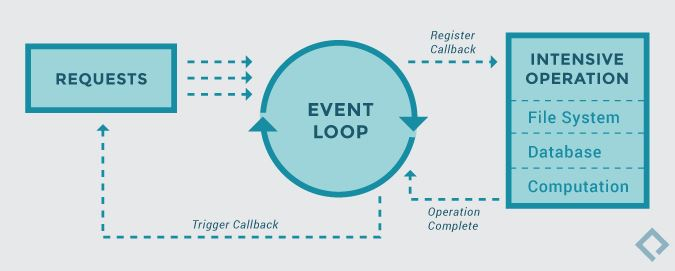
\includegraphics[width=4.4in]{figures/asyncio_process.jpg}
 \caption{AsyncIO mechanism; it provides a high-performance asynchronous frameworks for making our fuzzing requests ~\cite{asyncio_image_source}.}
 \label{fig:asyncio_image_source}
\end{figure}

Communication with the target's web site is achieved with a blazingly fast asynchronous http client/server framework named aiohttp ~\cite{aiohttp}. The aiohttp module creates a reusable Session object per web application through which all requests are performed. Since our fuzzer, works with one web application per execution, a single session is created, shared across all tasks, and reused for the entire execution of the program. The re-usability of the session is feasible because, all tasks are running on the same thread. The aiohttp paired with asyncio really speed things up.

It is important to note here that note all available Python modules are compatible with asyncio. For instance, for our requests, we could not use the default and recommended Python's requests package, since it is built on top of {\tt urllib3 }, which in turn uses Python's http and socket modules. Socket operations are blocking and not awaitable which means Python would not like the await statement. However, more and more modules are becoming compatible with asyncio ~\cite{aiohttp}.

\section{Parser}
The fuzzer's parsing module is responsible for extracting vital information during the fuzzing process from each response received, after of course the respective request was made. Each response contains the HTML document which is then parsed using the {\tt  Beautiful Soup}~\cite{beautiful_soup} module in order to extract the form and anchor elements from it. These elements are useful as they can provide us with new URLs which translates to potentially new code paths and bugs to further explore and find. When found, they are added to the crawler's pending request list, and if they happen to be interesting (see Section ~\ref{sec:architecture}) they will also be fuzzed in the future. At this stage the HTML document is also checked for XSS vulnerabilities. The metadata that we store for each request, can tell us which XSS payloads were injected into it and lead to this vulnerability. If they happen to reside in the HTML document, which signal an RXSS vulnerability, a warning is triggered, incrementing the total number of XSS found and logging the related information. The document is also checked for Stored XSS vulnerabilities by scanning the document for all the XSS payloads that we have injected in all requests so far. A high-level pseudocode for the parsing process can be seen at Algorithm ~\ref{alg:parser_pseudocode}. As the pseudocode shows clearly, parsing relies heavily on the urllib.parse~\cite{urllib_parse} Python module. This module, and more precisely the urlparse method, is used for breaking the Uniform Resource Locator (URL) string up in components; such as addressing scheme, network location, path etc. An object is return that contains 6-item tuple with all the URL sub-fields. The reverse can also be achieve through the urlunparse method; a URL object can be converted into string.

\begin{algorithm}
 
 \caption{Parsing new HTML documents method pseudocode.}
 \label{alg:parser_pseudocode}
 
 \begin{algorithmic}
	\STATE lookForXSS(HTML) \COMMENT{Increments global XSS counter if one is found.} 
	\STATE $links \leftarrow set()$ 
	\FOR{every form found in the HTML document}
		 \IF{form does \NOT contain an action field}
 			\STATE $urlObject \leftarrow urllib.parse(callingNodeUrl)$
		 \ELSE 
 			\STATE $urlObject \leftarrow urllib.parse(relativeToAbsolute(form.action))$
		 \ENDIF
		\STATE $parameters \leftarrow parseQueryString(urlObject.query)$ 
		\STATE $urlString \leftarrow urllib.unparse(urlObject)$ 
		\STATE $inputs \leftarrow dictionary()$ 
		\FOR{every < input > element found in form}
			\STATE $value \leftarrow input.get(value)$			 
	 		\STATE $name \leftarrow input.get(name)$	
	 		\STATE $inputs[name] \leftarrow append(value)$	 
		\ENDFOR
		\STATE $method \leftarrow form.get(method)$	
		\STATE $Node \leftarrow createNode(parameters, urlString, inputs, method)$	
		\STATE $links \leftarrow add(Node)$
		\FOR{every < a > element found in form}
			\STATE $anchor \leftarrow a.get(href)$			 
		\ENDFOR
		\STATE $Node \leftarrow createNode(parameters, urlString, inputs, method)$	
		\STATE $links \leftarrow add(Node)$
	\ENDFOR
	\RETURN links
 \end{algorithmic}
\end{algorithm}

\section{Curses Interface}
An textual user interfaces (TUI) for \pname{} has been created using the curses module which contains various information and essential statistics, gathered while our gray-box fuzzer is running. The curses library supplies a terminal-independent screen-painting and keyboard-handling facility for text-based terminals~\cite{curses}, such as the Linux console. The text editor nano is a good example of a curses application. As you can imagine, this functionality is not available for Windows, as the Windows version of Python does not include the curses module. So by running our fuzzing tool on a Windows based machine, regardless of the Command Line Interface (CLI) you opt to use, it will result in a crush. There are of-course ways to run \pname{} without this interface which will be elaborated in the next subsection. Although many may think this is an obsolete technology, it can prove to be quite valuable for Unix-based operating systems that do not provide any graphical support. The Python module, which is the one we utilise, is a fairly simple wrapper over the C functions provided by the first and original curses. A snapshot of the interface provided by webFuzz can be seen at Figure ~\ref{fig:curses_interface}. As the figure illustrates, statistics are divided in to three categories; namely the process statistics, the overall progress and the examining node details.
As the fuzzing tools expands, more and more valuable information will be included on the interface.

\begin{figure}[ht]
 \centering
 \captionsetup{justification=centering}
 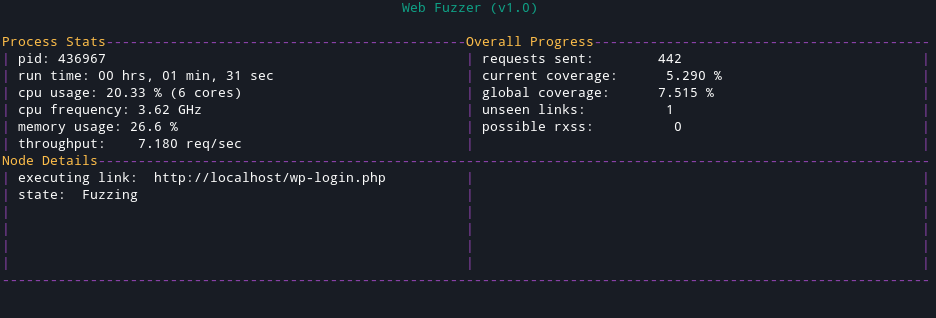
\includegraphics[width=4.6in]{figures/curses.png}
 \caption{A screenshot of the webFuzz interface. The interface is implemented using the Curses module.}
 \label{fig:curses_interface}
\end{figure}


\section{Running webFuzz}
Running \pname{} is fairly simple. All necessary modules accompanied with their exact version needed to be installed for \pname{} to work smoothly, are listed in a "requirements" text file. Other dependencies, executing and installing dependencies instructions can be found at the README.md file in the tool's repository. A help menu that shows all available arguments in which \pname{} can run in, are shown at Figure ~\ref{fig:argparser_menu}. As you can see, arguments are separated in three categories; namely optional, required and positional. Optional arguments are extra functionalities that you do not have to include when running the tool whereas required and positional are the arguments that must be included. For the creation of the usage menu and parsing the arguments, the argparse~\cite{argparse} Python module was used.
Also, throughout the execution, logging is used as a means of tracking events that happen when the fuzzer runs. Logging is a module in the Python standard library that provides a richly-formatted log.

\begin{figure}[ht]
 \centering
 \captionsetup{justification=centering}
 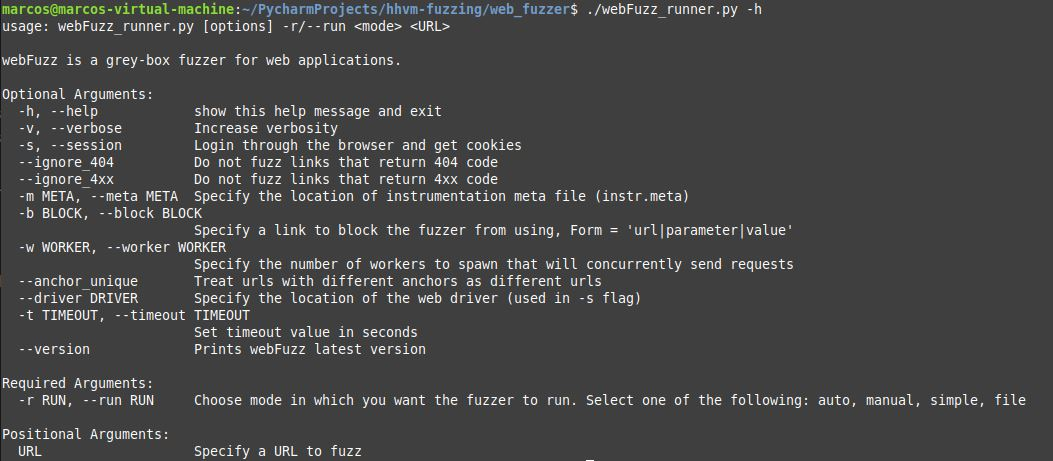
\includegraphics[width=4.6in]{figures/argparser_menu.jpg}
 \caption{\pname{} help menu includes all available arguments which we can use to run it with.}
 \label{fig:argparser_menu}
\end{figure}
